\section{Flow and Congestion Control (continued)}
\subsection{Congestion Control}
\subsection{Slow Start Implementation}
\begin{itemize}[nosep]
    \item Let $w$ be the size of the window in \emph{bytes}
          \begin{itemize}[nosep]
              \item We have $\sfrac{w}{\texttt{MSS}}$ segments per RTT
          \end{itemize}
    \item We are doubling $w$ after each RTT
          \begin{itemize}[nosep]
              \item We receive $\sfrac{w}{\texttt{MSS}}$ ACKs each RTT
              \item So we can set $w = w + \texttt{MSS}$ on every ACK
          \end{itemize}
    \item At some point, we hit the network limit
          \begin{itemize}[nosep]
              \item Experience loss
              \item We are at most one window size above the limit
              \item Remember this: \texttt{ssthresh} and reduce window
          \end{itemize}
\end{itemize}

\subsection{Slow Start}
\begin{itemize}[nosep]
    \item We double \texttt{cwnd} every round trip
    \item We are still sending $\min(\texttt{cwnd}, \texttt{rcvwnd})$ packets
    \item Continue until \texttt{ssthresh} estimate or packet drop
\end{itemize}

\subsection{Dealing with Congestion}
\begin{itemize}[nosep]
    \item Assume losses are due to congestion
    \item After a loss, reduce congestion window
          \begin{itemize}[nosep]
              \item \emph{How much to reduce?}
          \end{itemize}
    \item Idea: conservation of packets at equilibrium
          \begin{itemize}[nosep]
              \item Want to keep roughly the same number of packets network
              \item Analogy with water in fixed-size pipe
              \item Put new packet into network when one exits
          \end{itemize}
\end{itemize}

\subsection{How much to reduce window?}
\begin{itemize}[nosep]
    \item What happens under congestion?
          \begin{itemize}[nosep]
              \item Exponential increase in congestion
          \end{itemize}
    \item Sources must decrease offered rate exponentially
          \begin{itemize}[nosep]
              \item i.e., multiplicative decrease in window size
              \item TCP chooses to cut window in half
          \end{itemize}
\end{itemize}

\subsection{How to use extra capacity?}
\begin{itemize}[nosep]
    \item Network signals congestion, but says nothing of underitilization
          \begin{itemize}[nosep]
              \item Senders constantly try to send faster, see if it works
              \item So, increase window if no losses\dots By how much?
          \end{itemize}
    \item Multiplicative increase?
          \begin{itemize}[nosep]
              \item Easier to saturate the network than to recover
              \item Too fast, will lead to saturation, wild fluctuations
          \end{itemize}
    \item Additive Increase?
          \begin{itemize}[nosep]
              \item Won't saturate the network
          \end{itemize}
\end{itemize}

\subsection{Chiu Jain Phase Plots}
\begin{figure}[H]
    \tikzsetnextfilename{chiu-jain-fair}
    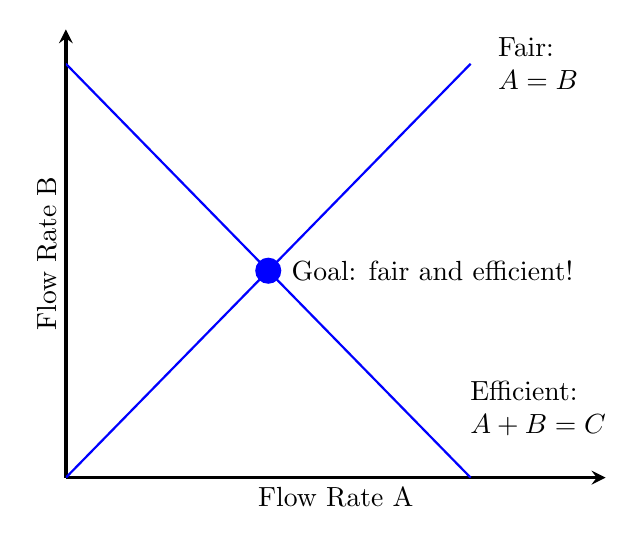
\begin{tikzpicture}
        \begin{axis}[
                xlabel = Flow Rate A,
                ylabel=Flow Rate B,
                xmin=-3,
                xmax=5,
                ymin=-3,
                ymax=3.5,
                axis lines = left,
                ticks=none,
                axis line style={very thick}
            ]
            \addplot[color=blue,domain=-3:3,thick]{x};
            \addplot[color=blue,domain=-3:3,thick]{-x};
            \node[circle, minimum size=1mm, fill=blue, label=right:{Goal: fair and efficient!}] at (0, 0) {};
            \node[align=left] at (4, 3) {Fair:\\$A=B$};
            \node[align=left] at (4, -2) {Efficient:\\$A + B = C$};
        \end{axis}
    \end{tikzpicture}
\end{figure}

\begin{figure}[H]
    \tikzsetnextfilename{mimd}
    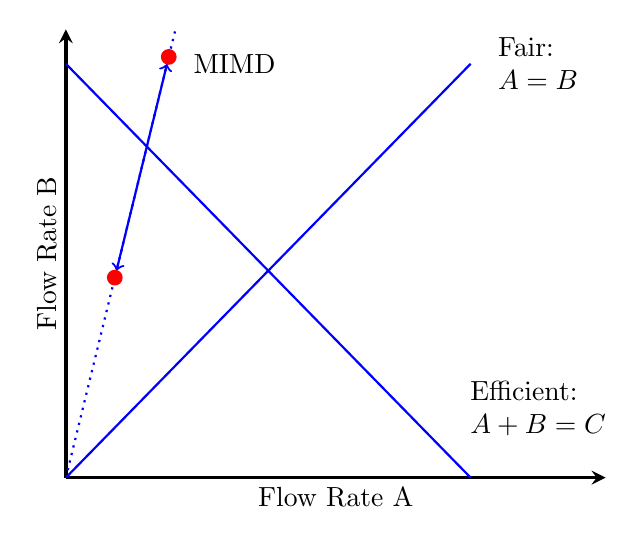
\begin{tikzpicture}
        \begin{axis}[
                xlabel = Flow Rate A,
                ylabel=Flow Rate B,
                xmin=-3,
                xmax=5,
                ymin=-3,
                ymax=3.5,
                axis lines = left,
                ticks=none,
                axis line style={very thick}
            ]
            \addplot[color=blue,domain=-2.25:-1.5,thick,<->]{4*x+9};
            \addplot[color=blue,domain=-3:3,thick]{x};
            \addplot[color=blue,domain=-3:3,thick]{-x};
            \addplot[color=blue,domain=-3:3,dotted,thick]{4*x+9};
            \node[align=left] at (4, 3) {Fair:\\$A=B$};
            \node[align=left] at (4, -2) {Efficient:\\$A + B = C$};
            \node[circle, minimum size=2mm, fill=red,inner sep=0] at (-2.275, -0.1) {};
            \node[circle, minimum size=2mm, fill=red,inner sep=0] at (-1.475, 3.1) {};
            \node at (-0.5, 3) {MIMD};
        \end{axis}
    \end{tikzpicture}
\end{figure}

\begin{figure}[H]
    \tikzsetnextfilename{aiad}
    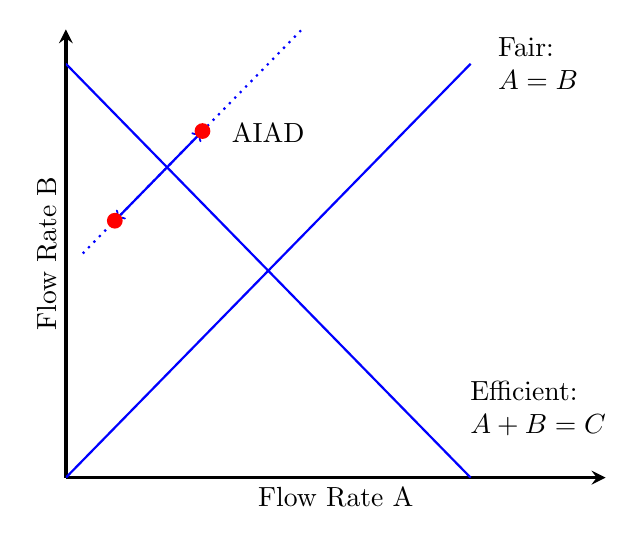
\begin{tikzpicture}
        \begin{axis}[
                xlabel = Flow Rate A,
                ylabel=Flow Rate B,
                xmin=-3,
                xmax=5,
                ymin=-3,
                ymax=3.5,
                axis lines = left,
                ticks=none,
                axis line style={very thick}
            ]
            \addplot[color=blue,domain=-2.25:-1,thick,<->]{x+3};
            \addplot[color=blue,domain=-3:3,thick]{x};
            \addplot[color=blue,domain=-3:3,thick]{-x};
            \addplot[color=blue,domain=-2.75:3,dotted,thick]{x+3};
            \node[align=left] at (4, 3) {Fair:\\$A=B$};
            \node[align=left] at (4, -2) {Efficient:\\$A + B = C$};
            \node[circle, minimum size=2mm, fill=red,inner sep=0] at (-2.275, 0.725) {};
            \node[circle, minimum size=2mm, fill=red,inner sep=0] at (-0.975, 2.025) {};
            \node at (0, 2) {AIAD};
        \end{axis}
    \end{tikzpicture}
\end{figure}

\begin{figure}[H]
    \tikzsetnextfilename{aimd}
    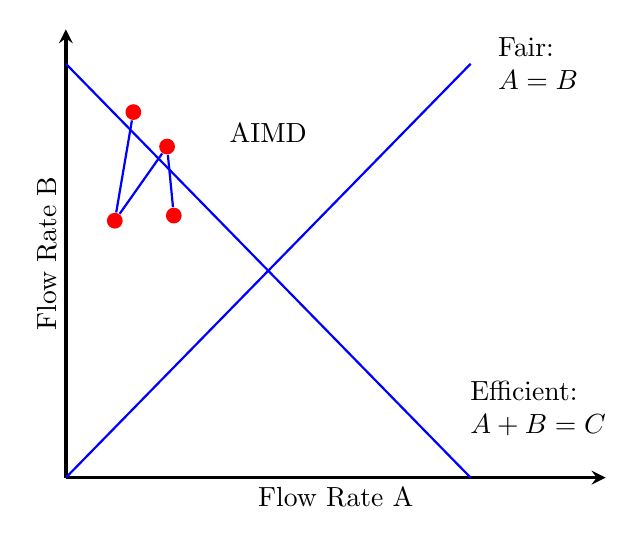
\begin{tikzpicture}
        \begin{axis}[
                xlabel = Flow Rate A,
                ylabel=Flow Rate B,
                xmin=-3,
                xmax=5,
                ymin=-3,
                ymax=3.5,
                axis lines = left,
                ticks=none,
                axis line style={very thick}
            ]
            \addplot[color=blue,domain=-3:3,thick]{x};
            \addplot[color=blue,domain=-3:3,thick]{-x};
            \node[align=left] at (4, 3) {Fair:\\$A=B$};
            \node[align=left] at (4, -2) {Efficient:\\$A + B = C$};
            \node[circle, minimum size=2mm, fill=red,inner sep=0] at (-2.275, 0.725) (p2) {};
            \node[circle, minimum size=2mm, fill=red,inner sep=0] at (-2, 2.3) (p1) {};
            \node[circle, minimum size=2mm, fill=red,inner sep=0] at (-1.5, 1.8) (p3) {};
            \node[circle, minimum size=2mm, fill=red,inner sep=0] at (-1.4, 0.8) (p4) {};

            \draw[blue,thick] (p1) -- (p2) -- (p3) -- (p4);

            \node at (0, 2) {AIMD};
        \end{axis}
    \end{tikzpicture}
\end{figure}

\subsection{AIMD Implementation}
\begin{itemize}[nosep]
    \item In practice, send \texttt{MSS}-sized segments
          \begin{itemize}[nosep]
              \item Let window size in bytes be $w$ (a multiple of \texttt{MSS})
          \end{itemize}
    \item Increase:
          \begin{itemize}[nosep]
              \item After $w$ bytes ACKed, could set $w = w + \texttt{MSS}$
              \item Smoother to increment on each ACK
                    \begin{itemize}[nosep]
                        \item $w = w + \texttt{MSS} \times \sfrac{\texttt{MSS}}{w}$
                        \item (receive $\sfrac{w}{\texttt{MSS}}$ ACKs per RTT, increase by $\frac{\texttt{MSS}}{\sfrac{w}{\texttt{MSS}}}$ for each)
                    \end{itemize}
              \item Decrease:
                    \begin{itemize}[nosep]
                        \item After a packet loss, $w = \sfrac{w}{2}$
                        \item But dont want $w < \texttt{MSS}$
                        \item So react differently to multiple consecutive losses
                        \item Back off exponentially (pause with no packets in flight)
                    \end{itemize}
          \end{itemize}
\end{itemize}

\subsection{AIMD Trace}
\begin{itemize}[nosep]
    \item AIMD produces sawtooth pattern of window size
          \begin{itemize}[nosep]
              \item Always probing available bandwidth
          \end{itemize}
\end{itemize}
\begin{figure}[H]
    \tikzsetnextfilename{aimd-bandwidth}
    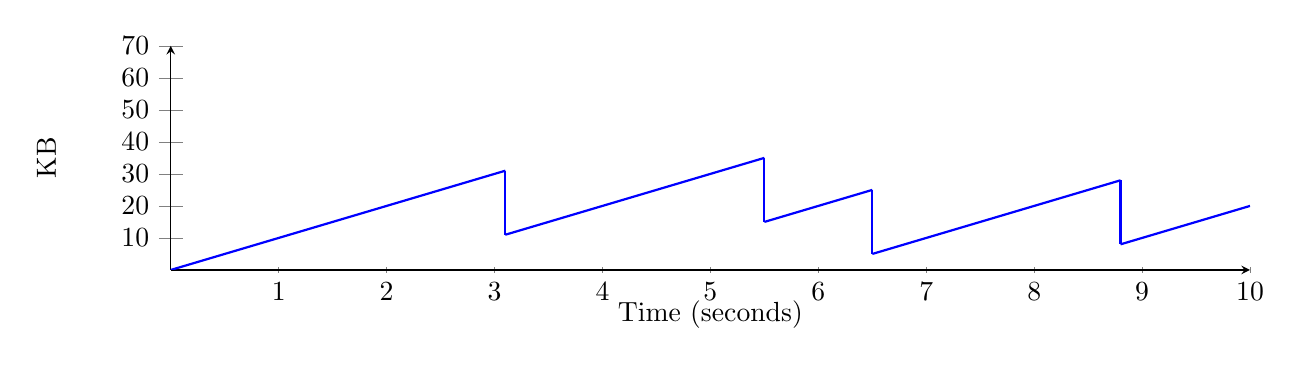
\begin{tikzpicture}
        \begin{axis}[
                xlabel = Time (seconds),
                ylabel=KB,
                xmin=0,
                xmax=10,
                xtick={1.0,2.0,3.0,4.0,5.0,6.0,7.0,8.0,9.0,10.0},
                ytick={10,20,30,40,50,60,70},
                ymin=0,
                ymax=70,
                axis lines = left,
                yscale=0.5,
                xscale=2,
            ]
            \addplot[color=blue,domain=0:3.1,thick]{10 * x};
            \addplot[color=blue,domain=3.1:5.5,thick]{10 * x - 20};
            \addplot[color=blue,domain=5.5:6.5,thick]{10 * x - 40};
            \addplot[color=blue,domain=6.5:8.8,thick]{10 * x - 60};
            \addplot[color=blue,domain=8.8:10,thick]{10 * x - 80};

            \draw[color=blue,thick] (3.1, 31) -- (3.1, 11);
            \draw[color=blue,thick] (5.5, 35) -- (5.5, 15);
            \draw[color=blue,thick] (6.5, 25) -- (6.5, 5);
            \draw[color=blue,thick] (8.8, 28) -- (8.8, 8);
        \end{axis}
    \end{tikzpicture}
\end{figure}

\subsection{Putting it Together}
\begin{itemize}[nosep]
    \item TCP has two states: Slow Start (SS) and Congestion Avoidance (CA)
    \item A window size threshold governs the state transition
          \begin{itemize}[nosep]
              \item Window $\leq$ threshold: SS
              \item Window $>$ threshold: CA
          \end{itemize}
    \item States differ in how they respond to ACK
          \begin{itemize}[nosep]
              \item Slow start $w = w + \texttt{MSS}$
              \item Congestion Avoidance: $w = w + \sfrac{\texttt{MSS}^2}{w}$ (1 \texttt{MSS} per RTT)
          \end{itemize}
    \item On loss event: set $w = 1$, slow start
\end{itemize}

\subsection{How to Detect Loss}
\begin{itemize}[nosep]
    \item Timeout
    \item Any other way?
          \begin{itemize}[nosep]
              \item Gap in sequence numbers at receiver
              \item Receiver uses cumulative ACKs: drops $\Rightarrow$ duplicate ACKs
          \end{itemize}
    \item 3 duplicate ACKs considered loss
\end{itemize}

\subsection{RTT}
\begin{itemize}[nosep]
    \item We want an estimate of RTT so we can know a packet was likely lost, and not just delayed
    \item \emph{Key for correct operation}
    \item Challenge: RTT can be highly variable
          \begin{itemize}[nosep]
              \item Both at long and short time-scales!
          \end{itemize}
    \item Both average and variance increase a lot with load
    \item Solution
          \begin{itemize}[nosep]
              \item Use exponentially weighted moving average (EWMA)
              \item Estimate deviation as well as expected value
              \item Assume packet is lost when time is well beyond reasonable deviation
          \end{itemize}
\end{itemize}

\subsection{Originally}
\begin{itemize}[nosep]
    \item $\texttt{EstRTT} = (1 - \alpha) \times \texttt{EstRTT} + \alpha\texttt{SampleRTT}$
    \item $\texttt{Timeout} = 2 \times \texttt{EstRTT}$
    \item Problem 1:
          \begin{itemize}[nosep]
              \item in case of retransmission, ACK corresponds to which send?
              \item Solution: only sample for segments with no retransmission
          \end{itemize}
    \item Problem 2:
          \begin{itemize}[nosep]
              \item does not take variance into account: too aggressive when there is more load!
          \end{itemize}
\end{itemize}
\subsection{Jacobson/Karels Algorithm (Taho)}
\begin{itemize}[nosep]
    \item $\texttt{EstRTT} = (1 - \alpha)\times\texttt{EstRTT} + \alpha\times\texttt{SampleRTT}$
          \begin{itemize}[nosep]
              \item Recommended $\alpha$ is $0.125$
          \end{itemize}
    \item $\texttt{DevRTT} = (1 - \beta)\times\texttt{DevRTT} + \beta\abs{\texttt{SampleRTT} - \texttt{EstRTT}}$
          \begin{itemize}[nosep]
              \item Recomended $\beta$ is $0.25$
          \end{itemize}
    \item $\texttt{Timeout} = \texttt{EstRTT} + 4\cdot\texttt{DevRTT}$
    \item For successive retransmissions: use exponential backoff
\end{itemize}
\subsection{Slow start every time?!}
\begin{itemize}[nosep]
    \item Losses have large effect on throughput
    \item Fast Recovery (TCP Reno)
          \begin{itemize}[nosep]
              \item Same as TCP Tahoe on Timeout: $w=1$, slow start
              \item On triple duplicate ACKs: $w = \sfrac{w}{2}$
              \item Retransmit missing segment (fast retransmit)
              \item Stay in Congestion Avoidance mode
          \end{itemize}
\end{itemize}
\subsection{3 Challenges Revisited}
\begin{itemize}[nosep]
    \item Determining the available capacity in the first place
          \begin{itemize}[nosep]
              \item Exponential increase in congestion window
          \end{itemize}
    \item Adjusting to changes in the available capacity
          \begin{itemize}[nosep]
              \item Slow probing, AIMD
          \end{itemize}
    \item Sharing capacity between flows
          \begin{itemize}[nosep]
              \item AIMD
          \end{itemize}
    \item Detecting Congestion
          \begin{itemize}[nosep]
              \item Timeout based on RTT
              \item Triple duplicate acknowledgements
          \end{itemize}
    \item Fast retransmit/Fast recovery
          \begin{itemize}[nosep]
              \item Reduces slow starts, timeouts
          \end{itemize}
\end{itemize}